\newcommand{\homedir}{/home/bscholtz/workspace/workspace-latex/2016-Design-Project/LATEX/}

%######################Preamble######################
\input{"\homedir preamble.tex"}

\newcommand{\coursecode}{EEE4036A}
\newcommand{\assignment}{Design Project (Team 14)}
\newcommand{\lecturer}{Riana Geschke}

\pagestyle{fancy}
\fancyhf{}
\rhead{Design Project}
\lhead{Team 14}
\cfoot{\thepage}

\begin{document}

%######################Title Page######################
\begin{titlepage} 

\includegraphics[width = 17cm]{images/uctbanner.png} \\

\begin{center}
\begin{LARGE}
Faculty of Engineering and the Built Environment \\
Department of Electrical Engineering \\
\end{LARGE}
\end{center}

\begin{center}  
\begin{Huge}
\textbf{\coursecode}\\
\bigskip
\bigskip
\hrule
\assignment \\
\end{Huge}

\vspace*{\fill}

\hrule
\begin{center}
\textbf{Benjamin Scholtz (SCHBEN011)\\
Jarushen Govender (GVNJAR002)\\
Isaac Lebogang Khobo (KHBISA001)\\
Nasko Stavrev (STVATA001)\\}
4$^{th}$ year BSc. (Eng.) Electrical Engineering Department\\
Lecturer: \lecturer \\
\today
\end{center}
\bigskip
\hrule

\end{center}
\end{titlepage}

%######################Contents######################

\newpage
%\section*{Contents}
%\addcontentsline{toc}{section}{Contents}  
\tableofcontents

%######################Plagiarism Dec.######################
\input{"\homedir plagiarism-declaration.tex"}

%######################Begin Content######################
\newcommand{\lsec}[1]{\normalsize{\textbf{#1}}\\}

\newpage

\section{TASK CLARIFICATION}
\subsection{Background}
UCT Upper campus has a number of parking areas for staff, students and visitors using cars to travel to campus. There are red, yellow, blue and unmarked bays on campus. In addition there are disabled and 
visitor parking bays on campus. These categories are assigned the highest priority. 

For every user, a parking category is assigned, and an associated annual fee is charged.  The purchase of a parking disk allows the staff member/student/visitor to search for a parking spot in the designated category on campus, but it is not guaranteed that one will be available, since parking bays are oversold. When arriving on campus, a driver of a car may spend some time searching for an available spot in the required category. Parking disks are generally linked to a person and only valid for the specific vehicle for which the disk has been purchased, except for student lift clubs.

The Traffic  Department  on  Upper  Campus  administrates  and  manages  all  aspects  related  to  parking  of vehicles.\cite{assignment}
 
\subsection{Problem Statement}
For  a  driver  entering  Upper  Campus  in  a  car,  it  is  not immediately  apparent  where  there  are  parking bays available.  This is a particular problem during peak times when a large number of cars arrive on campus, looking for parking at the same time. The design assignment is to solve this problem using the electrical engineering skills of each of the team members in your group.\cite{assignment}

The design assignment is:

\begin{itemize}
\item To provide information in an easily accessible format, to each driver of a car immediately on arrival on campus, on where all the vacant parking bays on campus are. This must be for the specific category of parking for this user.

\item To determine whether a vehicle is parked on a bay not designated for this user, for example a yellow disk holder parks on a red bay, or a visitor parks on a disabled parking bay, and make this available to the traffic department in real time.

\item To  allow electronic reconfiguration  of  traffic  bay allocations  on  special  occasions, for example during the summer school period, when there are many visitors requiring parking on campus.

\item To monitor and log the use of parking bays and the percentage of occupation of each parking area and make this available to the traffic department, for the purpose of planning.\cite{assignment}
\end{itemize}

\newpage
\section{CONTEXT OF DESIGN}
\subsection{Macroeconomic Factors}
STEEPLE.
\subsection{Microeconomic Factors}


\newpage
\section{DESIGN SPECIFICATION}
\subsection{Scope}
This specification covers the analysis, design, production timeline and considerations, and lifecycle of the upgraded UCT parking system. The specification is for a parking system on upper campus to be used primarily in allocated parking zones rather than dispersed parking bays. The parking system specifications aim to meet the requirements introduced in the client problem statement.

\subsection{Applicable Documents}
The following documents are applicable to the project and are of importance to the ultimate specifications of the project:
\begin{itemize}
\item Group Allocation
\item Group Project Assignment
\item Design Notes
\end{itemize}

\subsection{Characteristics}
\subsubsection{Functional Characteristics}
\lsec{Function 1: User interface} 
Information must be available in an easily accessible format to indicate to drivers where legal parking bays are located.

\lsec{Function 2: Vehicle location}
Real time location and classification of vehicles in UCT parking areas based on user parking privileges. 

\lsec{Function 3: System back-end}
Traffic department should be able to access data about vehicles and users on a database as well as reconfigure traffic bay allocations. The use of parking bays should be monitored and logged to be processed to show percentage occupation of parking area and get historical data.

\lsec{Interface Characteristics} 
Function 1, 2 and 3 should be linked with a wireless communication method.

\newpage
\subsubsection{Quality Assurance}
\lsec{Standards and Codes}
The design must meet the following standards and codes:
\begin{itemize}
\item IEEE Standards.
\item SABS Standards.
\item ICASA RF Regulations.
\item RF PCB Design Standards.
\end{itemize}

\lsec{Methods of Testing}
The design should be tested using the following method:
\begin{enumerate}
\item Periodic random parking bay testing.
\item HIL system testing.
\item Brute force user and operator interface testing.
\item Long term power system testing.
\item RF propagation testing.
\end{enumerate}

\lsec{Reliability Issues}

Reliability issues will arise in the following forms:

\begin{itemize}
\item Component quality standards.
\item Supplier reliability (especially for importing).
\item User familiarity with the system.
\item Unknown environment variables (RF signal propagation, mechanical obstructions etc.)
\item Unknown user variables (User behaviour etc.)
\end{itemize}

\newpage
\subsubsection{Timescale}
\lsec{Design Schedule}
The embodiment design should be completed within the given period of just under two months, in time for hand in after the first UCT term.

\lsec{Development Schedule}
Thereafter the final design should be developed and tested within a period of 4 months; and certified with the relevant organisations within a period of 2 months.

\lsec{Production Schedule}
The final design should be prototyped over a period of 1 month and then any necessary changes completed within 1 month thereafter - a final product will be sent for production over the course of 1 month. The necessary traffic department staff training and student/user familiarisation will be completed during the production time period over a period of 2 months.

\lsec{Delivery Schedule}
The complete system will be installed and in use over the period of 1 month. 

\begin{figure}[H]
 \begin{ganttchart}[x unit=10mm, y unit chart=0.8cm]{1}{12}
\gantttitle{\textbf{Year of Implementation (months)}}{12} \\
\gantttitlelist{1,...,12}{1} \\
\ganttgroup{Design Schedule}{1}{2} \\
\ganttbar[bar/.append style={fill=yellow}]{Embodiment Design}{1}{2} \\
\ganttgroup{Development Schedule}{3}{8} \\
\ganttbar[bar/.append style={fill=blue}]{Final Design}{3}{6} \\
\ganttbar{Certification}{7}{8} \\
\ganttgroup{Production Schedule}{9}{11} \\
\ganttbar[bar/.append style={fill=blue}]{Prototype and Testing}{9}{9} \\
\ganttbar{Final Changes}{10}{10} \\
\ganttbar[bar/.append style={fill=blue}]{Final Production}{11}{11} \\
\ganttbar[bar/.append style={fill=red}]{Training and Familiarisation}{9}{10} \\
\ganttgroup{Delivery Schedule}{12}{12} \\
\ganttbar[bar/.append style={fill=red}]{Installation}{12}{12} \\
%\ganttmilestone{Milestone}{11} \ganttnewline

\ganttlink{elem1}{elem3}
\ganttlink{elem3}{elem4}
\ganttlink{elem4}{elem6}
\ganttlink{elem6}{elem7}
\ganttlink{elem7}{elem8}
\ganttlink{elem2}{elem9}
\ganttlink{elem8}{elem11}
\end{ganttchart}
\caption{Project Gantt Chart.}
\end{figure}

\subsubsection{Economic Factors}
\lsec{Market Analysis}
To calculate the upper campus UCT parking cash flow in the table below, a few assumptions were made. Approximately 2.8 parking discs are allocated per bay. Assuming this is true of all parking bay categories, this results in a total cash flow of R13.6 million per year. Assuming that 20\% of this cash flow is used for maintenance, and the other 20\% for parking staff salaries, we are left with R8.16 million for the project, with possible external funding if necessary.

The following table shows the number of different privilege level parking spots  and what the user pay for those slots, as well as how many users are allocated to those spots in order to calculate the cash flow acquired from the user yearly disc payments.

\begin{table}[H]
\centering
\caption{Upper Campus UCT Parking Cash Flow}
\label{cash-flow}
\begin{tabular}{lllll}
                         & \textbf{Parking Bays} & \textbf{Allocated Bays} & \textbf{Disc Price (R)} & \textbf{Cash Flow (R)} \\
\textbf{Red}                      & 808                   & 2262.4                  & 1524                & 3447897.6          \\
\textbf{Yellow}          & 1046                  & 2928.8                  & 960                 & 2811648            \\
\textbf{Student}         & 2757                  & 7719.6                  & 960                 & 7410816            \\
\textbf{Total Bays}      & 4611                  & 12910.8                 &                     &                    \\
\textbf{}                &                       &                         &                     &                    \\
\textbf{Discs/bay}       & 2.8                   &                         &                     &                    \\
\textbf{Total Cash Flow} & R13670361.6            &                         &                     &                   
\end{tabular}
\end{table}

From the table above and with with calculated R8.16 million available for research and development, the project capital expenditure should be below R5 million - this leaves enough capital for unforeseen expenses, either from oversight or incurred risk.

\lsec{Design Costs}
The design costs will be kept to a minimum by using UCT Electrical Engineering students to complete the design as a part of their EEE4036A design course.

\lsec{Development, Manufacturing, Distribution Costs}
The main costs incurred will be in contracted manufacturing and distribution. 

The following companies will be contracted to:
\begin{enumerate}
\item Zytek will be used for the manufacturing and assembly of the PCBs.
\item Skeg product development will be used for the tag and beacons casing production using injection mould methods.
\item Electronic components will be imported from Mouser predominantly. 
\end{enumerate}

The costs of development, manufacturing and distribution through the above sources should be kept to a unit cost value of less than R400 per tag. This ensures the cost of a disc will cover the cost of production of the tag, assuming  the allocation of funds as outlined above, with 60\% being left for hardware and software costs.

\newpage
\subsubsection{Ergonomic Factors}
\textit{\textbf{Device definition:} in the following sections a device refers to whatever user interface and necessary user interactions, whether with software or hardware, are required for the parking system.}

\lsec{User needs}
The user should be able to easily use the interface, whether internal (cellphone app etc.) or external (LED sign board) while driving. The use of the system should not endanger the user by distraction or otherwise. The device should not interfere with the users field of vision.

\lsec{Ergonomics}
The ergonomics of the device should meet the needs of the user. The interface should be easily accessible. The process of installing the device in the car should be self explanatory and not involve a complex process that requires assistance from UCT parking staff.

\lsec{Controls}
The controls of the device should meet the needs of the user. The controls should be minimal to avoid complexity and distraction, yes should also allow access to all the functions as set out above in the Functional Characteristics section.
\subsubsection{Life-cycle}
\lsec{Distribution}
Distribution of the device should be on a yearly basis, with user returning the device for maintenance and license renewal.

\lsec{Operation}
The user should be able to install the device easily and have it operate reliably for the period of one year. 

\lsec{Maintenance}
Minimal maintenance (whether for power source or mechanical maintenance or UID configuration) should be required for the device, with a minimum maintenance cycle of one year which is the period a user will be in possession of said device and expect it to operate reliably. Realistically this mean the maintenance cycle should be at least two years for worst case design - this will lessen the risk of a failure during the one year cycle.

\lsec{Disposal}
The device and it's components should, if required to be, be disposed of in a safe manner - this includes batteries and any other harmful substances. The device, after one year of use, should be returned to the parking staff especially during the initial testing phase where the system will be reviewed.

\newpage
\subsection{Acceptance Test Requirements}
\lsec{Function Test Requirements}
Test methods: Could be by inspection, theoretical modelling, simulation, laboratory functional demonstration, field trials, in-service measurements, etc.

\newpage
\section{CONCEPTUAL DESIGN}
\subsection{Design One}
Design One (D1) uses a triangulation system to locate the registered vehicle within the parking area. Each registered vehicle has a tag with a unique ID - this ID has the user data linked to it in a database on the server back-end. The location of each parking space is known, and with the knowledge of where the vehicle is located it can be determined whether the vehicle is legally parked or not. 
  
\subsubsection{System Diagram}
\subsubsection{System Components}
\lsec{Tags and Beacons}
Due to a triangulation system being used, in every parking area there are at least three beacons - with four being used to try to eliminate signal propagation issues. The tags and beacons make use of a Decawave DW1000 ultra-wideband transceiver chip that is controlled via SPI from a Atmel micro-controller. 

The master beacon sends a signal out to synchronise all the beacons to the same time reference. Each tag sends a signal periodically with the unique user ID, transmit time and battery level which is received by each of the beacons. The beacons all relay time of flight data back to the master beacon which performs a time difference of arrival (TDOA) calculation to determine where the tag is located.\cite{decawave-presentation}

The tags transmit with a period of 5-10 minutes. This reduces power consumption and signal noise level interference with other tags. The tags do not receive data. The tags will be accurate to within 10cm giving more than enough accuracy for the application. The initial conservative battery life estimate is 5 years with proper power management in software. They will be powered with a LiPo battery that will need to be replaced or charged when discharged.

The beacons will use the same circuitry, but with different software running on the Atmel micro-controller. They will be required to both transmit and receive. The beacons will be mounted on poles (both light and installed) distributed across the UCT campus - this will allow the location of vehicles in any area. They will be powered with LiPo batteries which will be charged with solar panels - or wired in cases where this is not practical.

\lsec{Server Back-end}
The server back-end connects with the master beacon via WiFi and receives the tag location, unique ID and battery level for every new vehicle. This is updated on a database every 5-10 minutes. Further calculations and visualizations are performed and stored in the database to send to the end user. The following data will be available for each unique ID:

\begin{itemize}
\item User privileges.
\item Tag location (updated periodically).
\item Tag battery level (updated periodically).
\end{itemize}

\lsec{User Interface}
The user interface will connect with the server back-end to access the database and will relay the following data to the end user via a smart phone application or web application: 
\begin{itemize}
\item Indication of privilege level and violations.
\item Tag battery level.
\item Vehicle location.
\item Location of open parking bays.
\item Recommended parking area.
\item Number of free parking bays in parking area.
\item Traffic heat-map on campus.
\end{itemize}

\subsubsection{Requirement Satisfaction\cite{assignment}}
Design One satisfies the design requirements outlined in the Task Clarification section in the following ways:

\begin{itemize}
\item \textbf{To provide information in an easily accessible format, to each driver of a car immediately on arrival on campus, on where all the vacant parking bays on campus are. This must be for the specific category of parking for this user.}

\item \textbf{To determine whether a vehicle is parked on a bay not designated for this user, for example a yellow disk holder parks on a red bay, or a visitor parks on a disabled parking bay, and make this available to the traffic department in real time.}

\item \textbf{To allow electronic reconfiguration  of  traffic  bay allocations on special occasions, for example during the summer school period, when there are many visitors requiring parking on campus.}

\item \textbf{To monitor and log the use of parking bays and the percentage of occupation of each parking area and make this available to the traffic department, for the purpose of planning.}
\end{itemize}

\subsubsection{Evaluation}
\lsec{Cost} 
(implementation, maintenance, energy consumption) \\
\lsec{Strong/weak Points}

\subsubsection{Risk Assessment}
\lsec{External Causes} 
(weather, vehicle impact, human interference) \\
risk of failure during intended life \\
\lsec{Internal Causes}
(Failure to recognize long-term design flaws)
\lsec{Mitigation}
mitigation (steps you will take to reduce the risk) \\

\subsection{Design Two}
\subsubsection{System Diagram}
\subsubsection{System Components}
\subsubsection{Requirement Satisfaction}

\subsubsection{Evaluation}
\lsec{Cost} 
(implementation, maintenance, energy consumption) \\
\lsec{Strong/weak Points}

\subsubsection{Risk Assessment}
\lsec{External Causes} 
(weather, vehicle impact, human interference) \\
risk of failure during intended life \\
\lsec{Internal Causes}
(Failure to recognize long-term design flaws)
\lsec{Mitigation}
mitigation (steps you will take to reduce the risk) \\

\newpage
\subsection{Weighted Selection}
The following weighted selection tables were formed and weights given to each aspect of the system design in order to determine which design meets the requirements outlined in the design specification:

\begin{table}[H]
\centering
\caption{Weighted selection: Design One\cite{handout}}
\label{weighted-selection-1}
\begin{tabular}{l|l|l|l|}
\textbf{Aspect}                      & \textbf{Score (1-5)} & \textbf{Weight} & \textbf{Total} \\ \hline
Functionality / User satisfaction    & 5                     & 20                & 20               \\
Cost of implementation / Maintenance & 5                     & 40                & 40               \\
Reliability / Safety                 & 4                     & 10                & 8                \\
Ease of installation / Maintenance   & 5                     & 20                & 20               \\
Life span                            & 3                     & 10                & 6                \\ \hline
\textbf{Total score (100):}          &                       &                   & 94              
\end{tabular}
\end{table}

\begin{table}[H]
\centering
\caption{Weighted selection: Design Two\cite{handout}}
\label{weighted-selection-2}
\begin{tabular}{l|l|l|l|}
\textbf{Aspect}                      & \textbf{Score (1-5)} & \textbf{Weight} & \textbf{Total} \\ \hline
Functionality / User satisfaction    & 3                     & 20                & 12               \\
Cost of implementation / Maintenance & 3                     & 40                & 24               \\
Reliability / Safety                 & 4                     & 10                & 8                \\
Ease of installation / Maintenance   & 4                     & 20                & 16               \\
Life span                            & 4                     & 10                & 8                \\ \hline
\textbf{Total score (100):}          &                       &                   & 68              
\end{tabular}
\end{table}

\subsection{Recommendation}
Based on the weighted selection and evaluation above, Design One should be further developed as a viable parking system solution for UCT upper campus. The embodiment design should be completed along with the necessary analysis and system testing.

\newpage
\section{EMBODIMENT DESIGN}
\subsection{System Overview}
\subsubsection{System Description}
\subsubsection{System Diagram}
\subsection{System Analysis}
Analysis of system operation, interfaces, use etc.
\subsection{Software Design}
\subsection{Mechanical Design} 
\subsubsection{Mechanical Requirements}
Durability, forces, dynamics.
\subsubsection{Technical Drawings}
\subsection{Electrical Design} 
\subsubsection{Power Requirements}
Battery life etc.

\newpage
\subsubsection{Schematics}

The following diagrams cover the design of the tag; where the beacon makes a few changes to the circuitry and adds a WiFi module, seen in Figure 5.

\begin{figure}[H]
\begin{center}
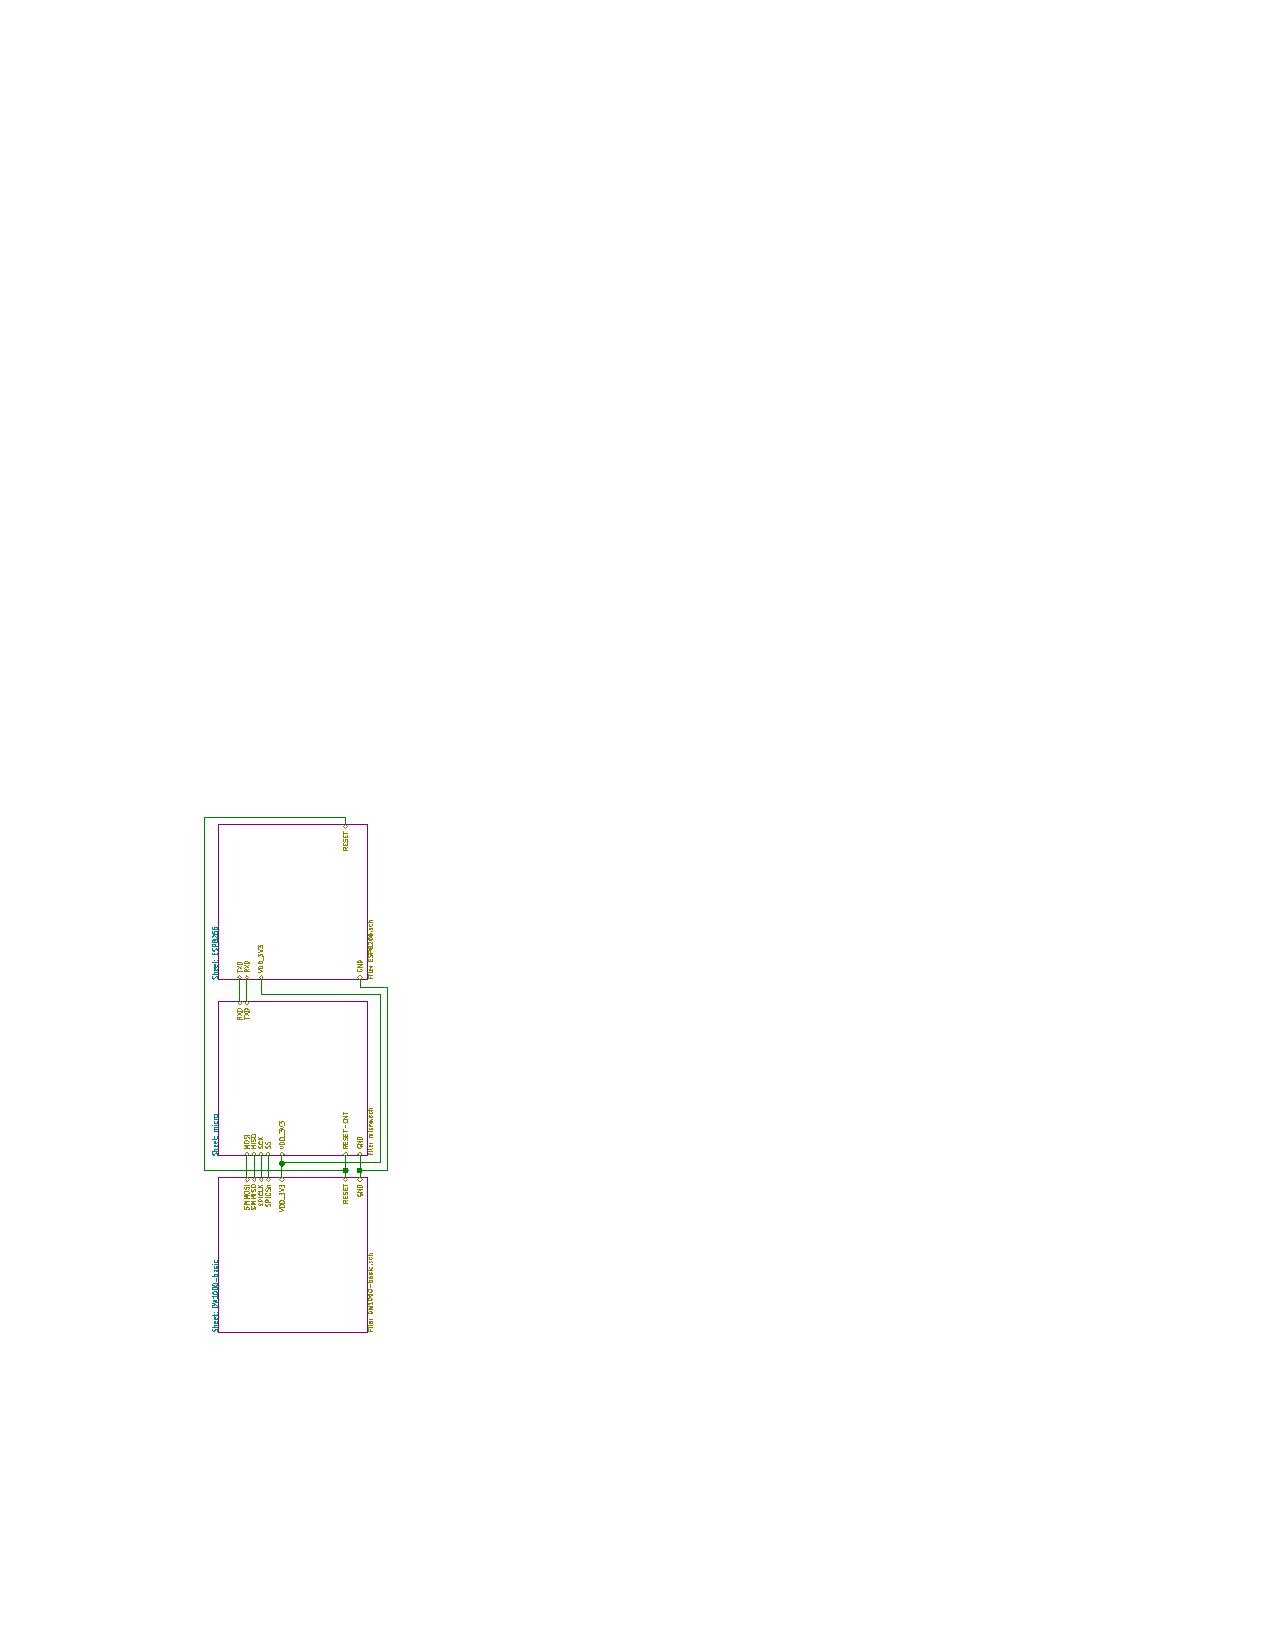
\includegraphics[page=1,scale=1.5,trim={3cm 5cm 15cm 13cm},clip,angle=-90]{data/parking-system2.pdf}
\caption{Parking system tag schematic diagram: interface connections.}
\end{center}
\end{figure}

\begin{figure}[H]
\begin{center}
\includegraphics[page=2,scale=0.5,trim={0cm 0cm 0cm 0cm},clip]{data/parking-system.pdf}
\caption{Parking system tag schematic diagram: transceiver chip.}
\end{center}
\end{figure}

\begin{figure}[H]
\begin{center}
\includegraphics[page=3,scale=1,trim={10cm 8cm 10cm 5cm},clip]{data/parking-system.pdf}
\caption{Parking system tag schematic diagram: micro-controller.}
\end{center}
\end{figure}

\begin{figure}[H]
\begin{center}
\includegraphics[page=4,scale=1,trim={5cm 9cm 10cm 13cm},clip,angle=-90]{data/parking-system2.pdf}
\caption{Parking system beacon schematic diagram: WiFi module.}
\end{center}
\end{figure}

\newpage
\subsubsection{PCB Design}

EMF and RF mitigation techniques have to be considered when designing the PCBs in order to make them compliant with the ICASA regulations. This involved using a ground plane and ensuring the antennas are correctly matched ($100\omega$ traces) to reduce RF harmonic signals.

\begin{figure}[H]
\begin{center}
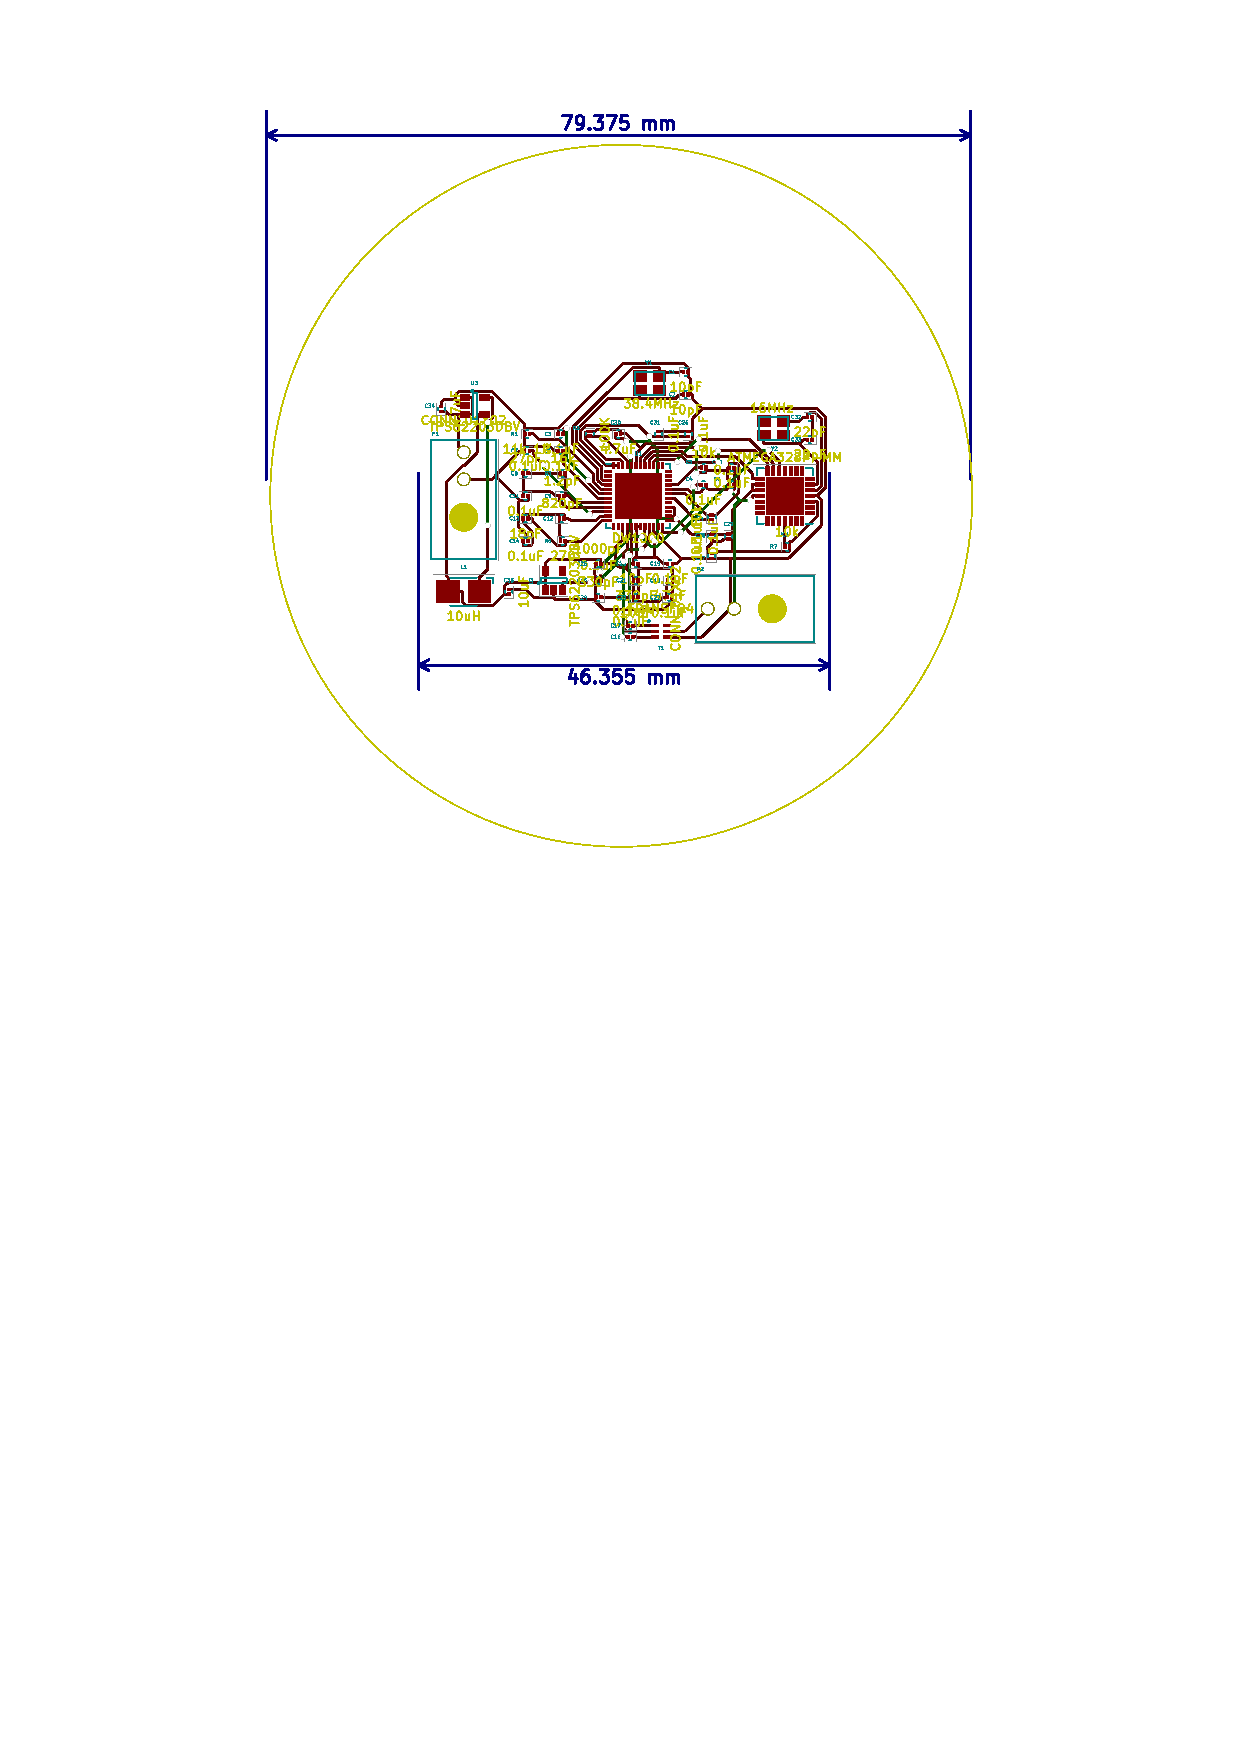
\includegraphics[scale=0.7,trim={4cm 15cm 4cm 1cm},clip]{data/pcb-layout.pdf}
\caption{Parking system tag PCB layout.}
\end{center}
\end{figure}

\begin{figure}[H]
\begin{center}
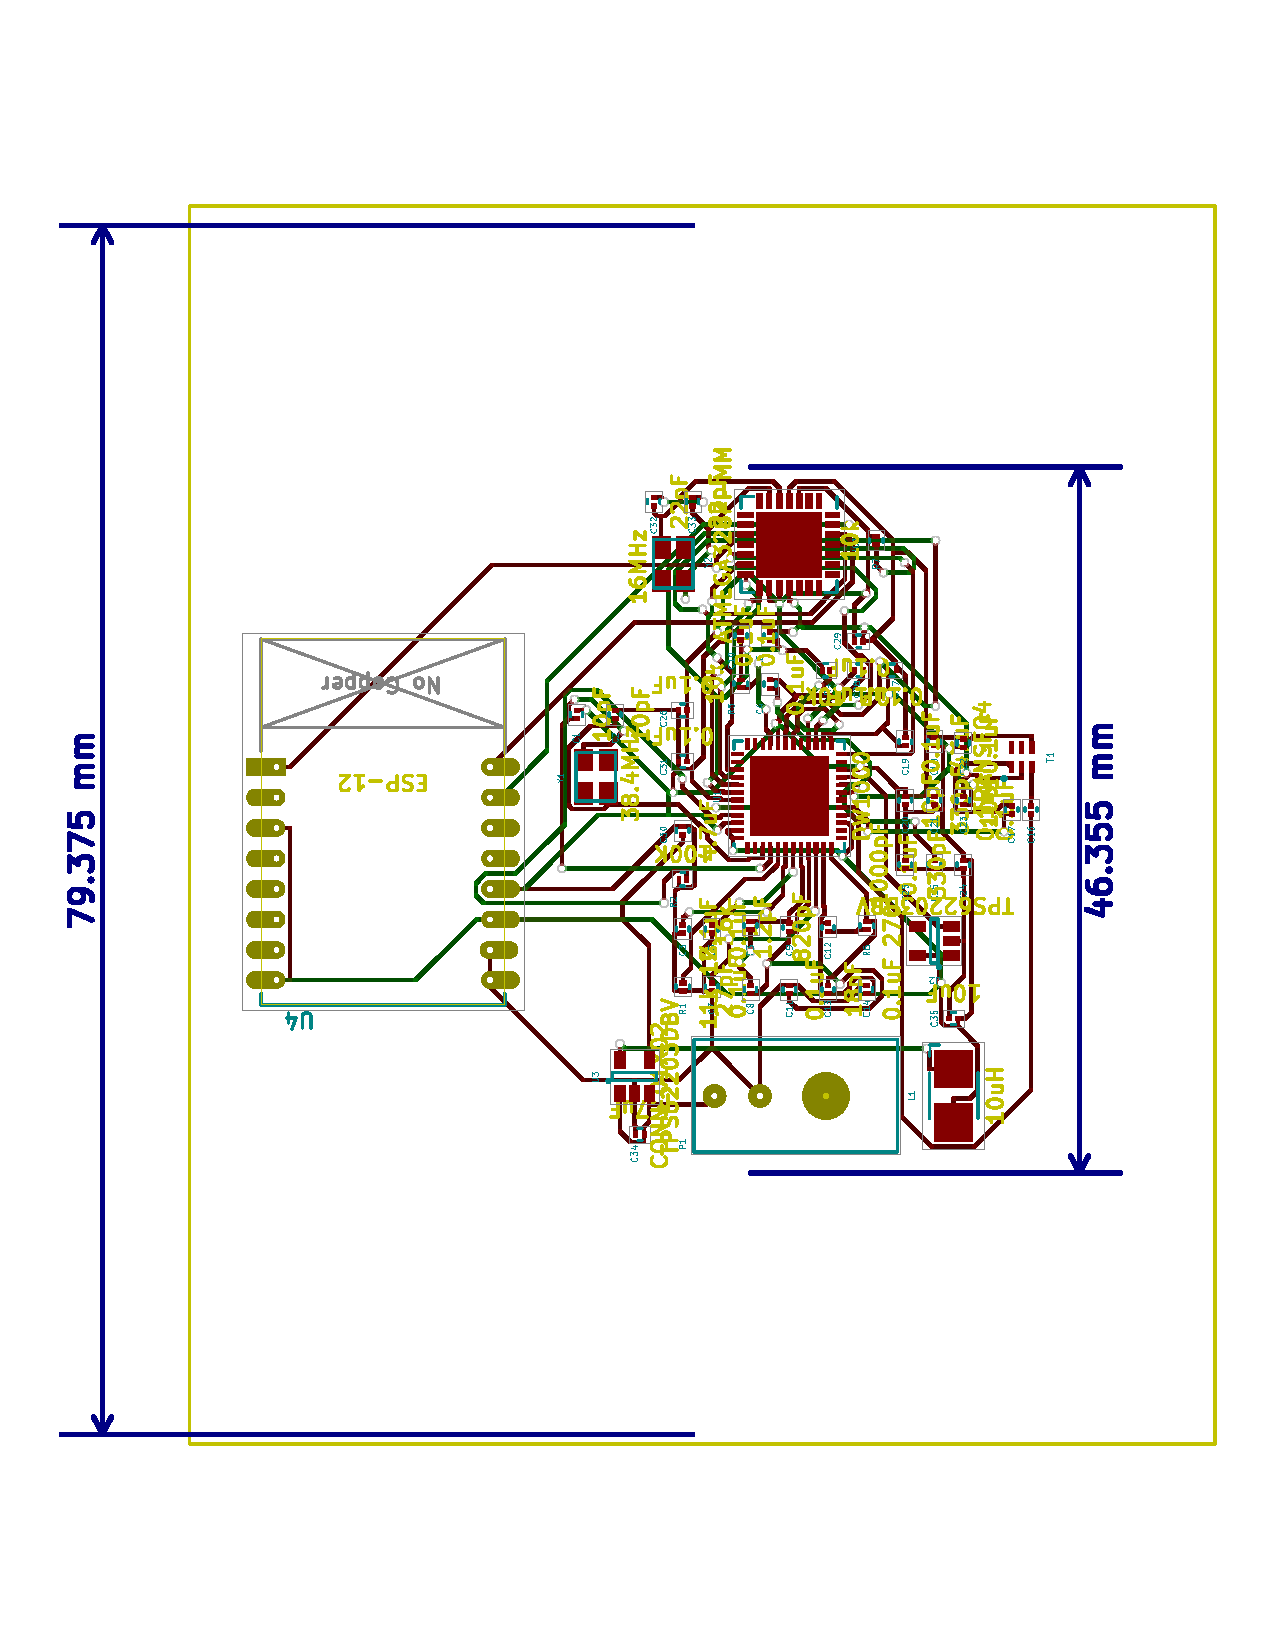
\includegraphics[scale=0.4,trim={1cm 1cm 1cm 1cm},clip,angle=-90]{data/pcb-layout-ESP.pdf}
\caption{Parking system beacon PCB layout.}
\end{center}
\end{figure}



\newpage
\subsubsection{RF Design}


\lsec{Antenna Specifciations:\cite{DW-antenna}}

Friss's Transmission Equation states the following:
$$P_{RX} = \frac{P_{TX}G_{TX}G_{RX} \lambda^2}{(4 \pi r)^2}$$
There is a quadratic relationship between the received power ($P_{RX}$) and the distance r from the tag to the beacon. This means we need to optimize the received power in another way, as the distance r can not be optimized except by having a dense beacon installation. The transmit power ($P_{TX}$) needs to be kept as low as possible, to optimize battery usage - this means the transmit and received antenna gain need to be made as high as is possible. The tag has a limited space profile, which means the beacon antenna needs to be as large as possible. Unfortunately the beacon antenna needs to be fairly omni-directional in order to pick up all the tags, as will be explained below, this further limits the possible receiver gain.

Because the antenna gains are measured using decibels which are on a logarithmic scale, the following changes in the equation need to be made:

$$P_{RX} = P_{TX} + G_{TX} + G_{R} + 20log_{10}(\frac{\lambda}{4 \pi R})$$


We would like to achieve at least a 60 percent transmission efficiency (this means 60 percent of the transmitted power is received) with a target of 90 percent efficiency. Designing for a 75 percent efficiency will help us achieve this target: 

$$\lambda = \frac{300e6}{f} = \frac{300e6}{3GHz} = 0.1m$$

$$EIRP(f) = P_{TX}G_{TX} = -41.3dBm/MHz$$
\begin{center}
value as mentioned below in regulations. This means the peak transmitter power and peak transmitter antenna gain must give a product within the regulations.
\end{center}

$$\frac{P_{RX}}{P_{TX}} = 0.75 = \frac{G_{TX}G_{RX} \times 0.1}{(4 \pi \times 200)^2} = $$

$$0.75 = 1 + G_{TX}$$

\begin{table}[H]
\centering
\caption{Antenna specifications: tag and beacon}
\label{antenna-specs}
\begin{tabular}{l l l l}
\textbf{Aspect}                      & \textbf{Tag} & \textbf{Beacon} \\ 
Radiation Pattern    	& Isotropic             & Dipole              \\
Power Output 			& 5                     & 40                     \\
Gain                 	& 2.6dBi                     & 10                    \\
Physical Area 			& 8mm					 & $1m^2$          \\         
Location 				& Mobile                & Fixed                    \\         
\end{tabular}
\end{table}

The tag antenna specifications are based on the calculations above and using the AH086M555003 PCB chip antenna from Mouser which has a wide operating range from 3100MHz to 8000MHz.

\lsec{ICASA National Radio Frequency Plan:\cite{ICASA}\cite{UWB-Regs}}
The ICASA 2013 NRFP for ITU Region 1 allocates the frequency range from 3.3GHz to 3.4GHz to radio-location with a typical application of government services. In South Africa there are no specific regulations for UWB signals. The Decawave technology is ETSI compliant and will generally be accepted by ICASA so long as EMF and RF mitigation techniques are used. The regulations permit outdoor use on the frequency range 3.1-4.8GHz with an EIRP of -41.3dBm/MHz. The ETSI regulations permit the use of the Decawave chips in an indoor and outdoor environment.

\lsec{DW1000 Frequency Channels:\cite{DW-antenna}}
The DW1000 can be programmed to use specific frequency channels (defined by the IEEE 802.15.4a-2011 standard) with corresponding bandwidth. Based on the ICASA regulations above, Channel 1 would be used with a Centre Frequency of 3493.4MHz and an operational bandwidth of 500MHz. This falls within the informal regulations mentioned above. 

\newpage
\subsubsection{Bill of Materials (Tag)}
The bill of materials as well as unit pricing for the tag can be found in Appendix C. Where parts with specific tolerance, such as for the RF circuitry, are needed they have been ordered specifically. The non-critical parts were chosen to optimize the end unit price. 

All parts were ordered from Mouser except if specified otherwise. They offer international shipping and are a reliable source of components to minimize risk. The LiPo batteries were ordered from a chinese source, as stated in the BOM, and the supplier will need to be managed properly to reduce risk.

\textbf{The result of the BOM and Unit Cost analysis is the following:}

Total Capital Outlay (ZAR): \\
Unit Cost (ZAR):

It was decided not to include the BOM and Unit Cost analysis for the beacons, as their costs will be minimal when compared with the 15000 tags needed for the system. In terms of circuitry, the beacons will work out to the same price as a tag - adding WiFi but not using LiPo batteries. There will be the additional expense of the following:

\begin{itemize}
\item WiFi chips
\item Beacon platform
\item Beacon power supplies
\item Antenna 
\end{itemize}

\subsection{Assumptions}
Identify and show that checked validity.
\subsection{Failure Modes}
Probabilities,Consequences,Mitigation
\subsection{System Lifetime}
A statement of the design life time, with explanation of what (if anything) will limit it.
\subsection{Worst Case Calculation}
For at least one component / sub-system 

\textit{Report structure compiled from class notes.}\cite{handout}\cite{notes}

%\begin{figure}[H]
%\begin{center}
%\includegraphics[trim={Lcm Bcm Rcm Tcm},clip]{images/Fig1.pdf}
%\caption{•}
%\end{center}
%\end{figure}

%\begin{minted}[linenos=true]{matlab}
%\end{minted}

%######################References######################
\newpage
%\input{"\homedir references.tex"} %manual references

\bibliography{bibliography}
\bibliographystyle{ieeetran}
\addcontentsline{toc}{section}{References}


%######################Appendices######################
\newpage
\vspace*{\fill}
\begin{center}
\subsection*{Appendix A: Contributions}
\end{center}
\vspace*{\fill}
\addcontentsline{toc}{section}{Appendix A: Contributions}

\newpage
\subsubsection*{Jarushen Govender (GVNJAR002)}
\subsubsection*{Isaac Lebogang Khobo (KHBISA001)}
\subsubsection*{Benjamin Scholtz (SCHBEN011)}
LATEX Formatting/Template. \\
2. Task Clarification. \\
4. Design Specification: Scope, Applicable Documents, Quality Assurance, Timescale, Economic Factors. \\
5. Conceptual Design: Design One, Weighted Selection, Recommendation. \\
6. Embodiment Design: Schematics, PCB Design, RF Design, Bill of Materials (Tag). \\
\subsubsection*{Nasko Stavrev (STVATA001)}

\newpage
\vspace*{\fill}
\begin{center}
\subsection*{Appendix B: Progress Reports}
\end{center}
\vspace*{\fill}
\addcontentsline{toc}{section}{Appendix B: Progress Reports}

\newpage
\vspace*{\fill}
\begin{center}
\subsection*{Progress Report 1: SCHBEN011}
\end{center}
\vspace*{\fill}
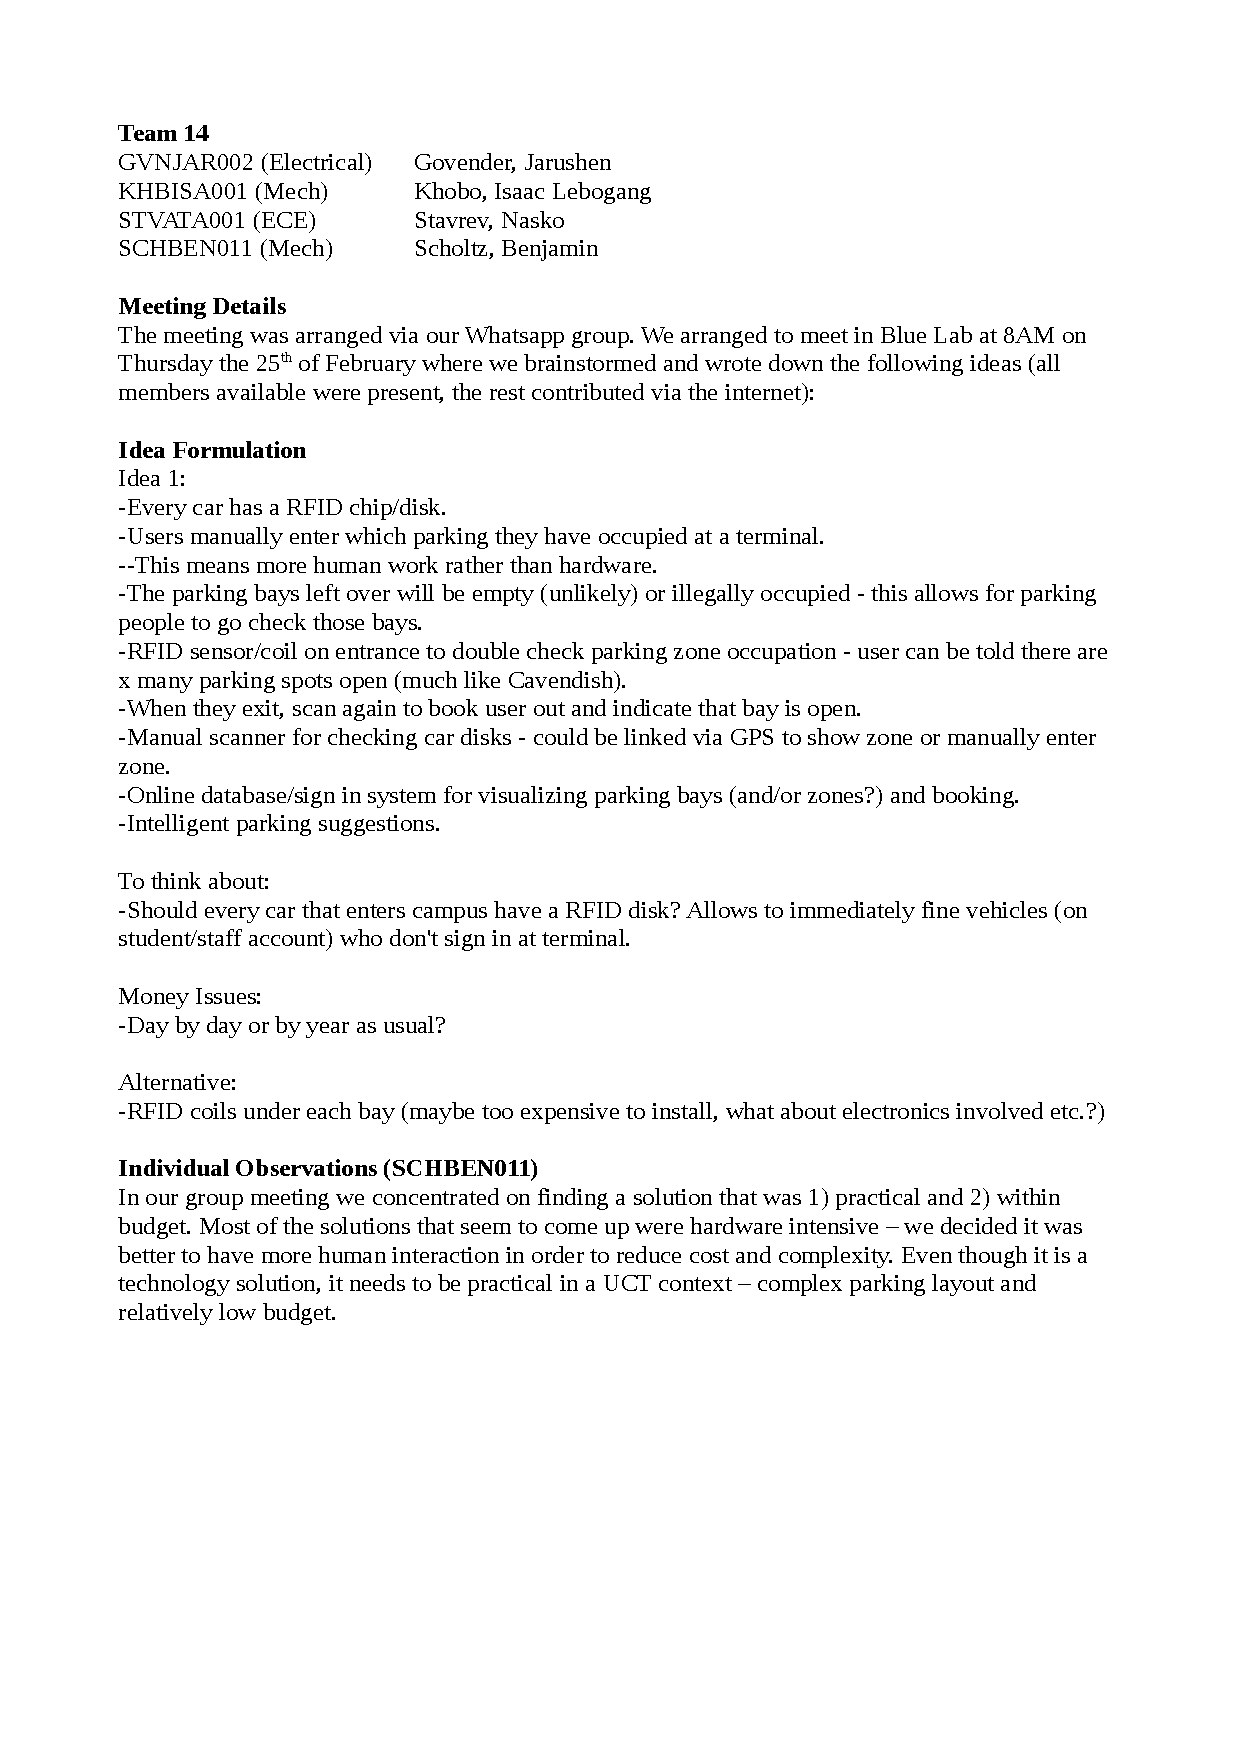
\includepdf[pages=-]{meeting/report1-ben.pdf}

\newpage
\vspace*{\fill}
\begin{center}
\subsection*{Progress Report 1: STVATA001}
\end{center}
\vspace*{\fill}
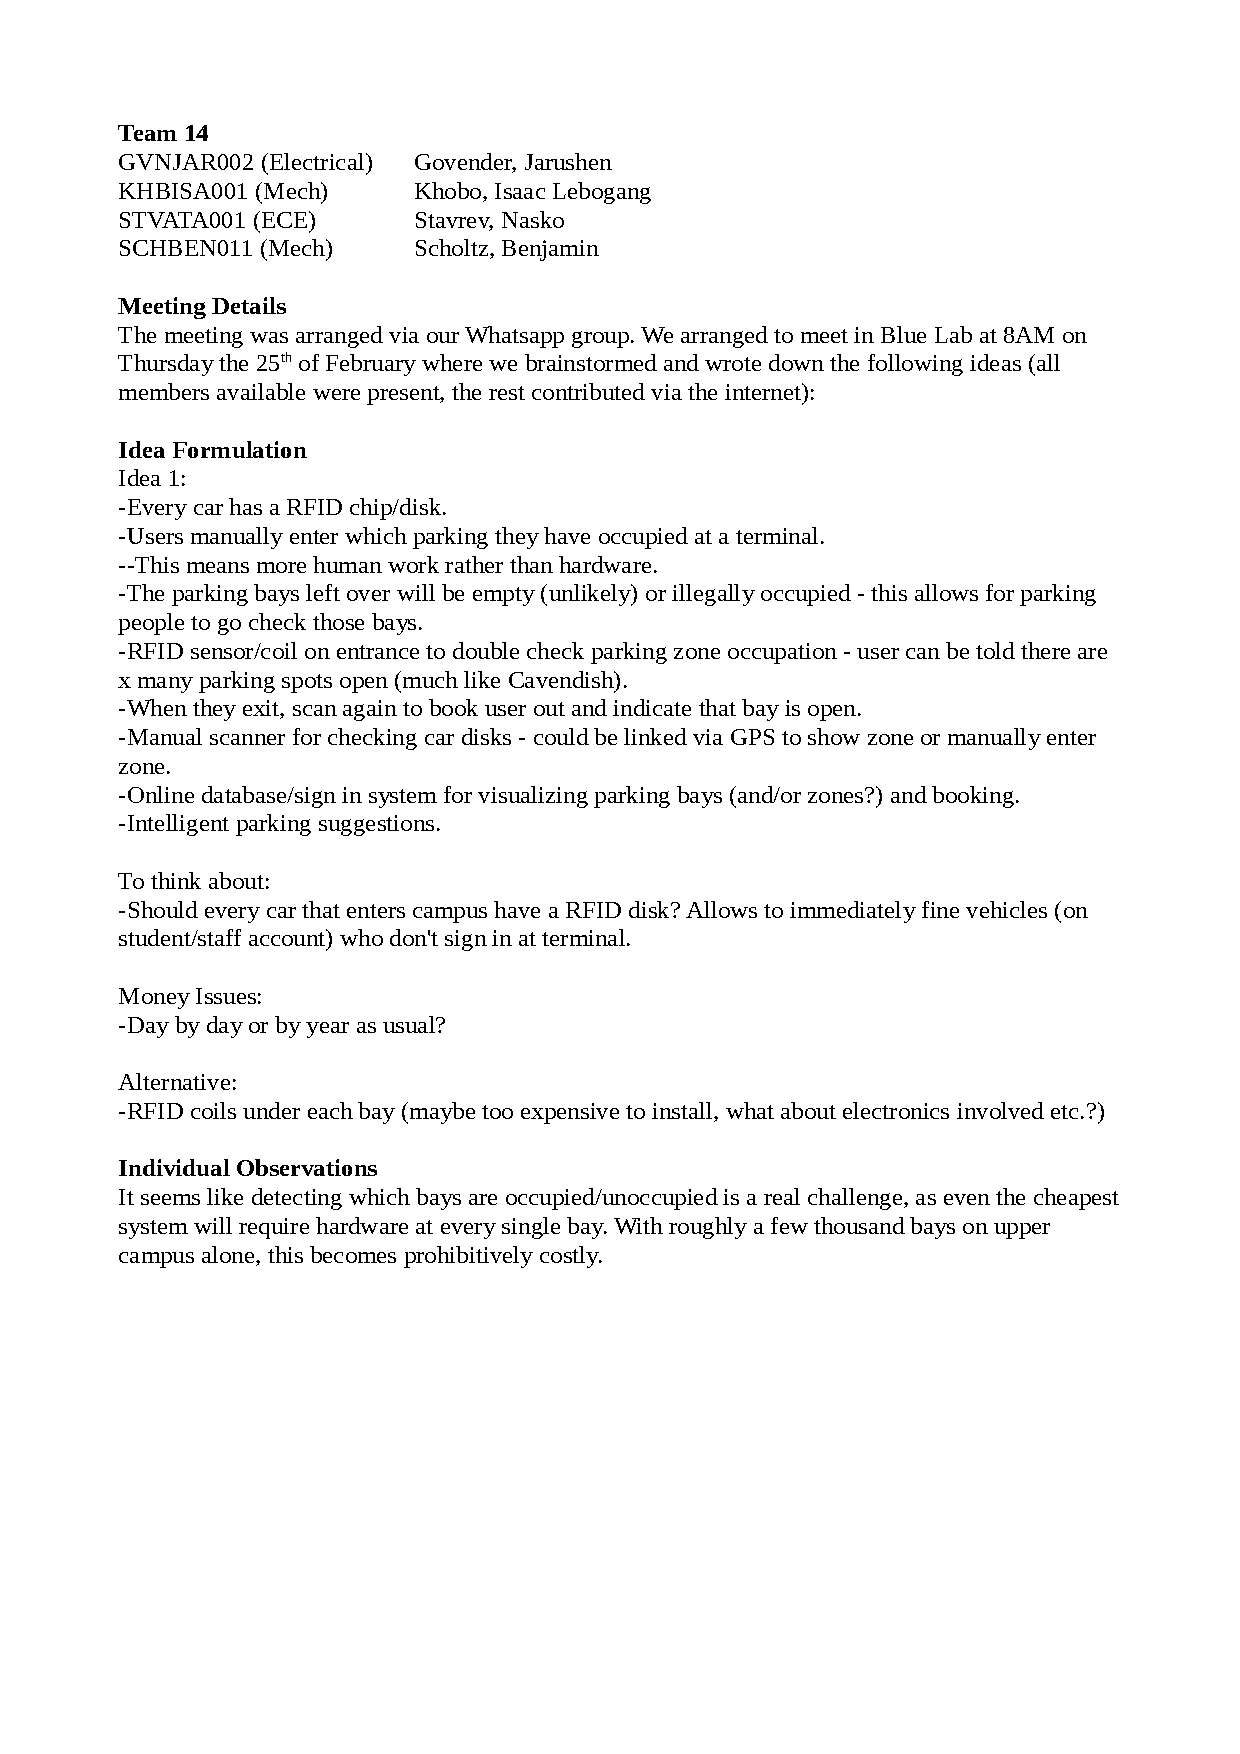
\includepdf[pages=-]{meeting/report1-nasko.pdf}

\newpage
\vspace*{\fill}
\begin{center}
\subsection*{Progress Report 1: KHBISA001}
\end{center}
\vspace*{\fill}
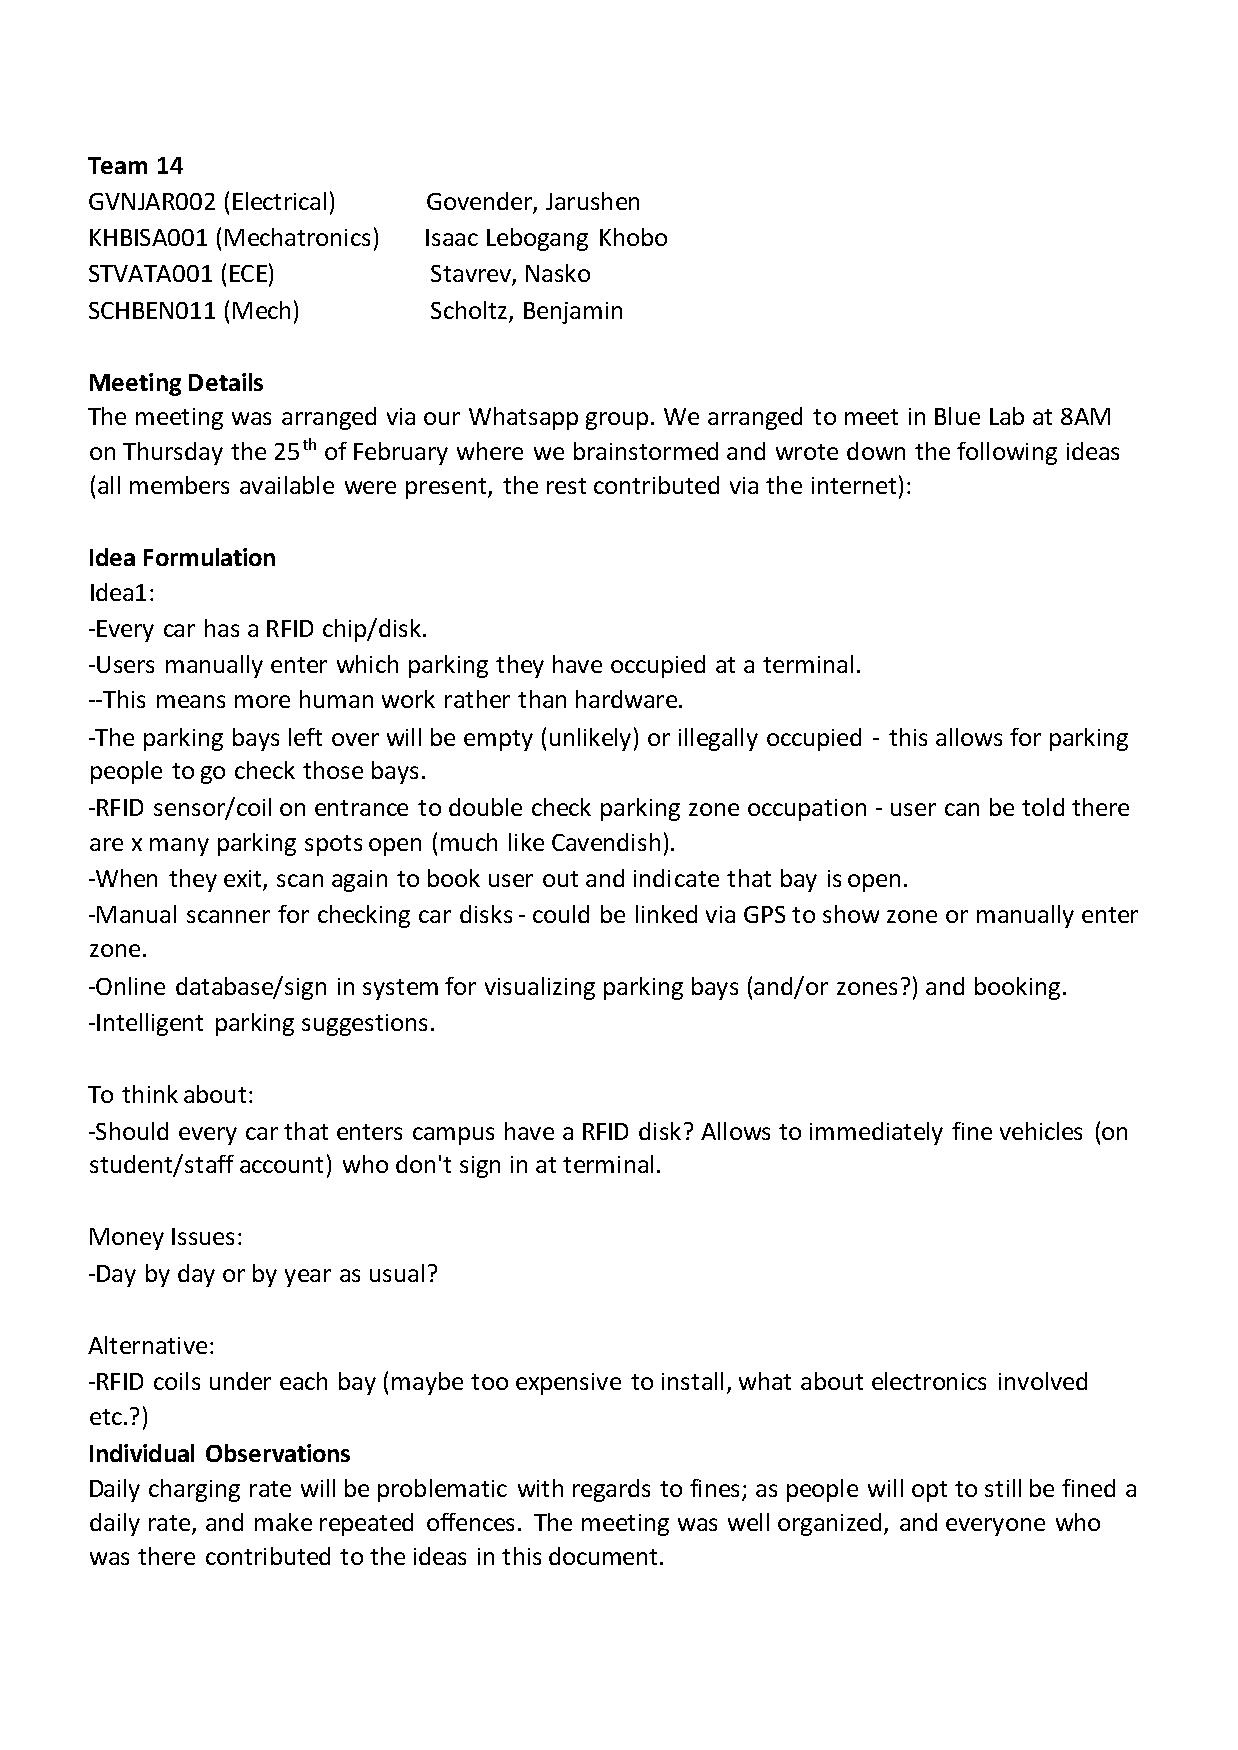
\includepdf[pages=-]{meeting/report1-isaac.pdf}

\newpage
\vspace*{\fill}
\begin{center}
\subsection*{Progress Report 1: GVNJAR002}
\end{center}
\vspace*{\fill}
%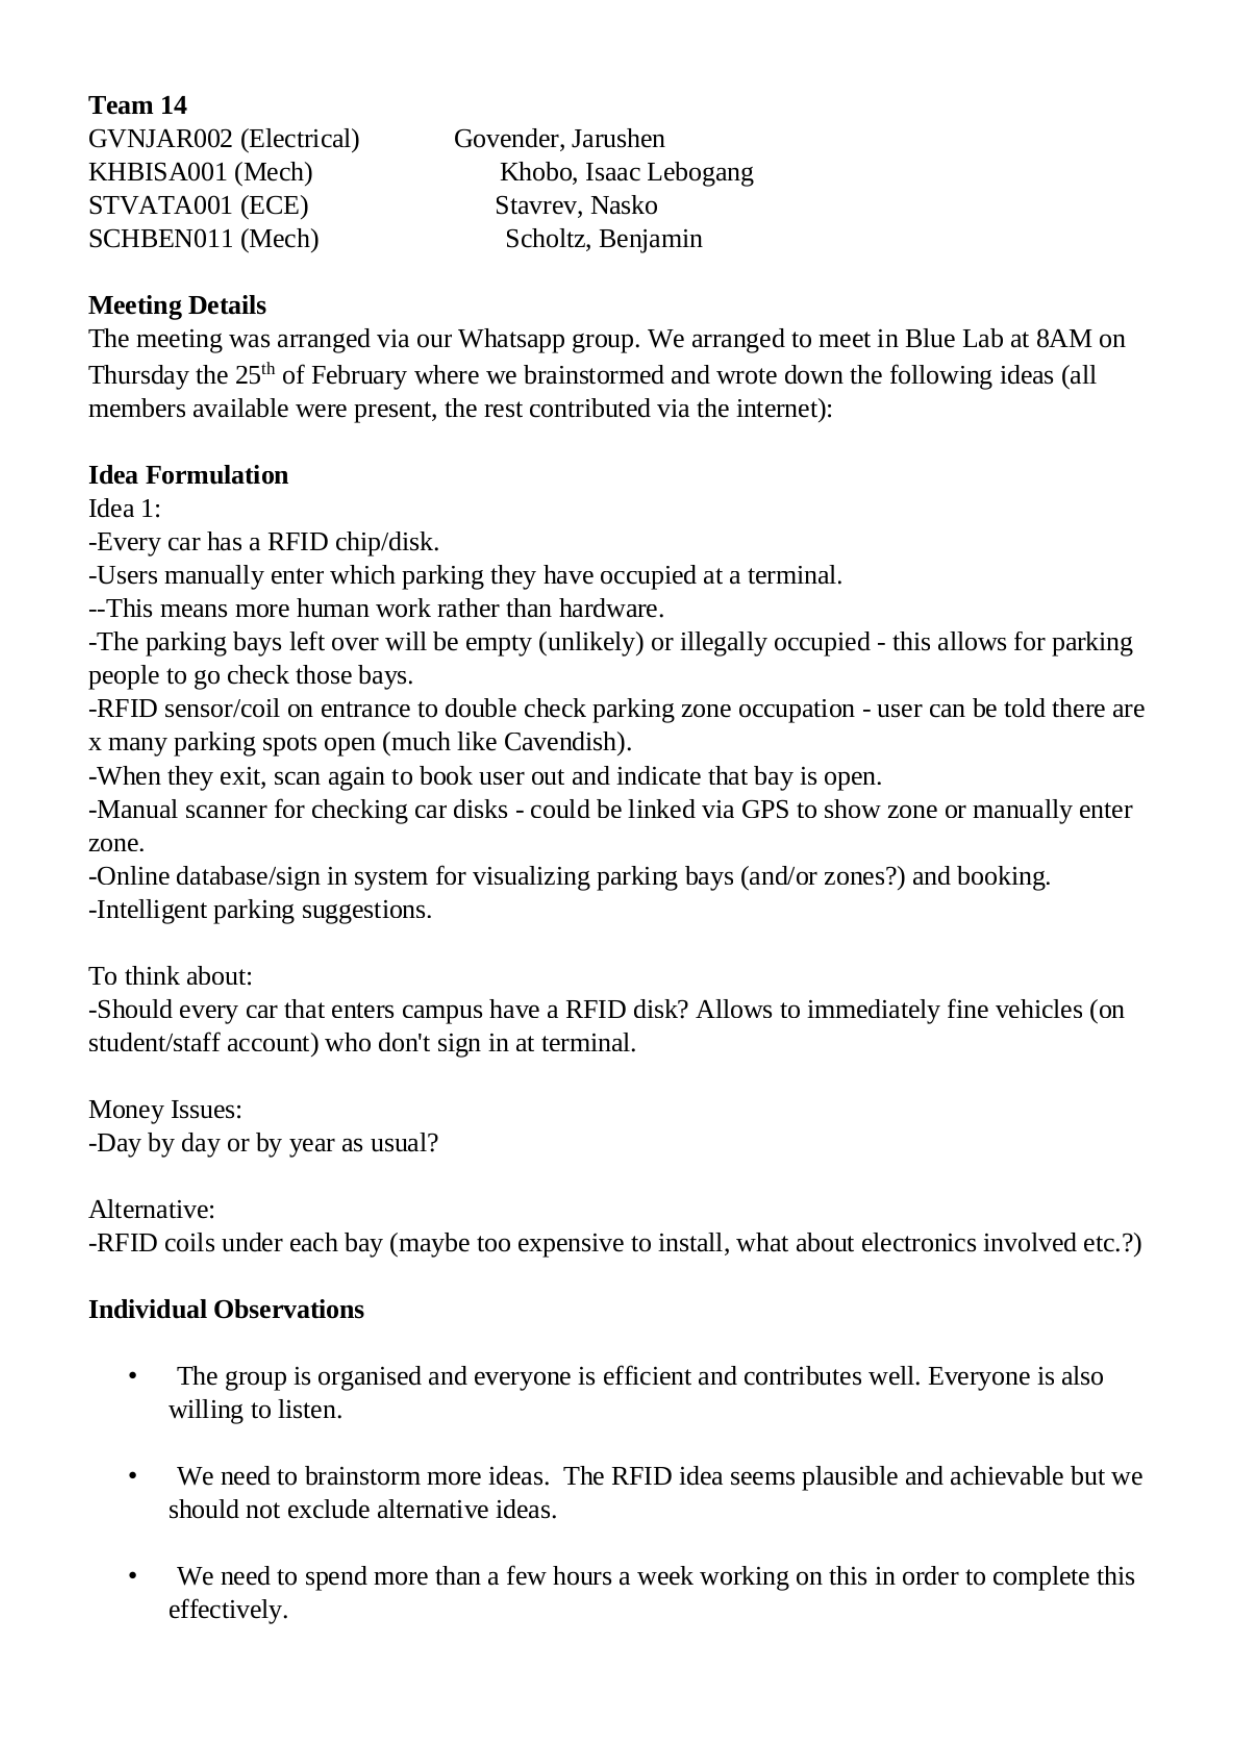
\includepdf[pages=-]{meeting/report1-jarushen.pdf}

\newpage
\vspace*{\fill}
\begin{center}
\subsection*{Progress Report 2}
\end{center}
\vspace*{\fill}
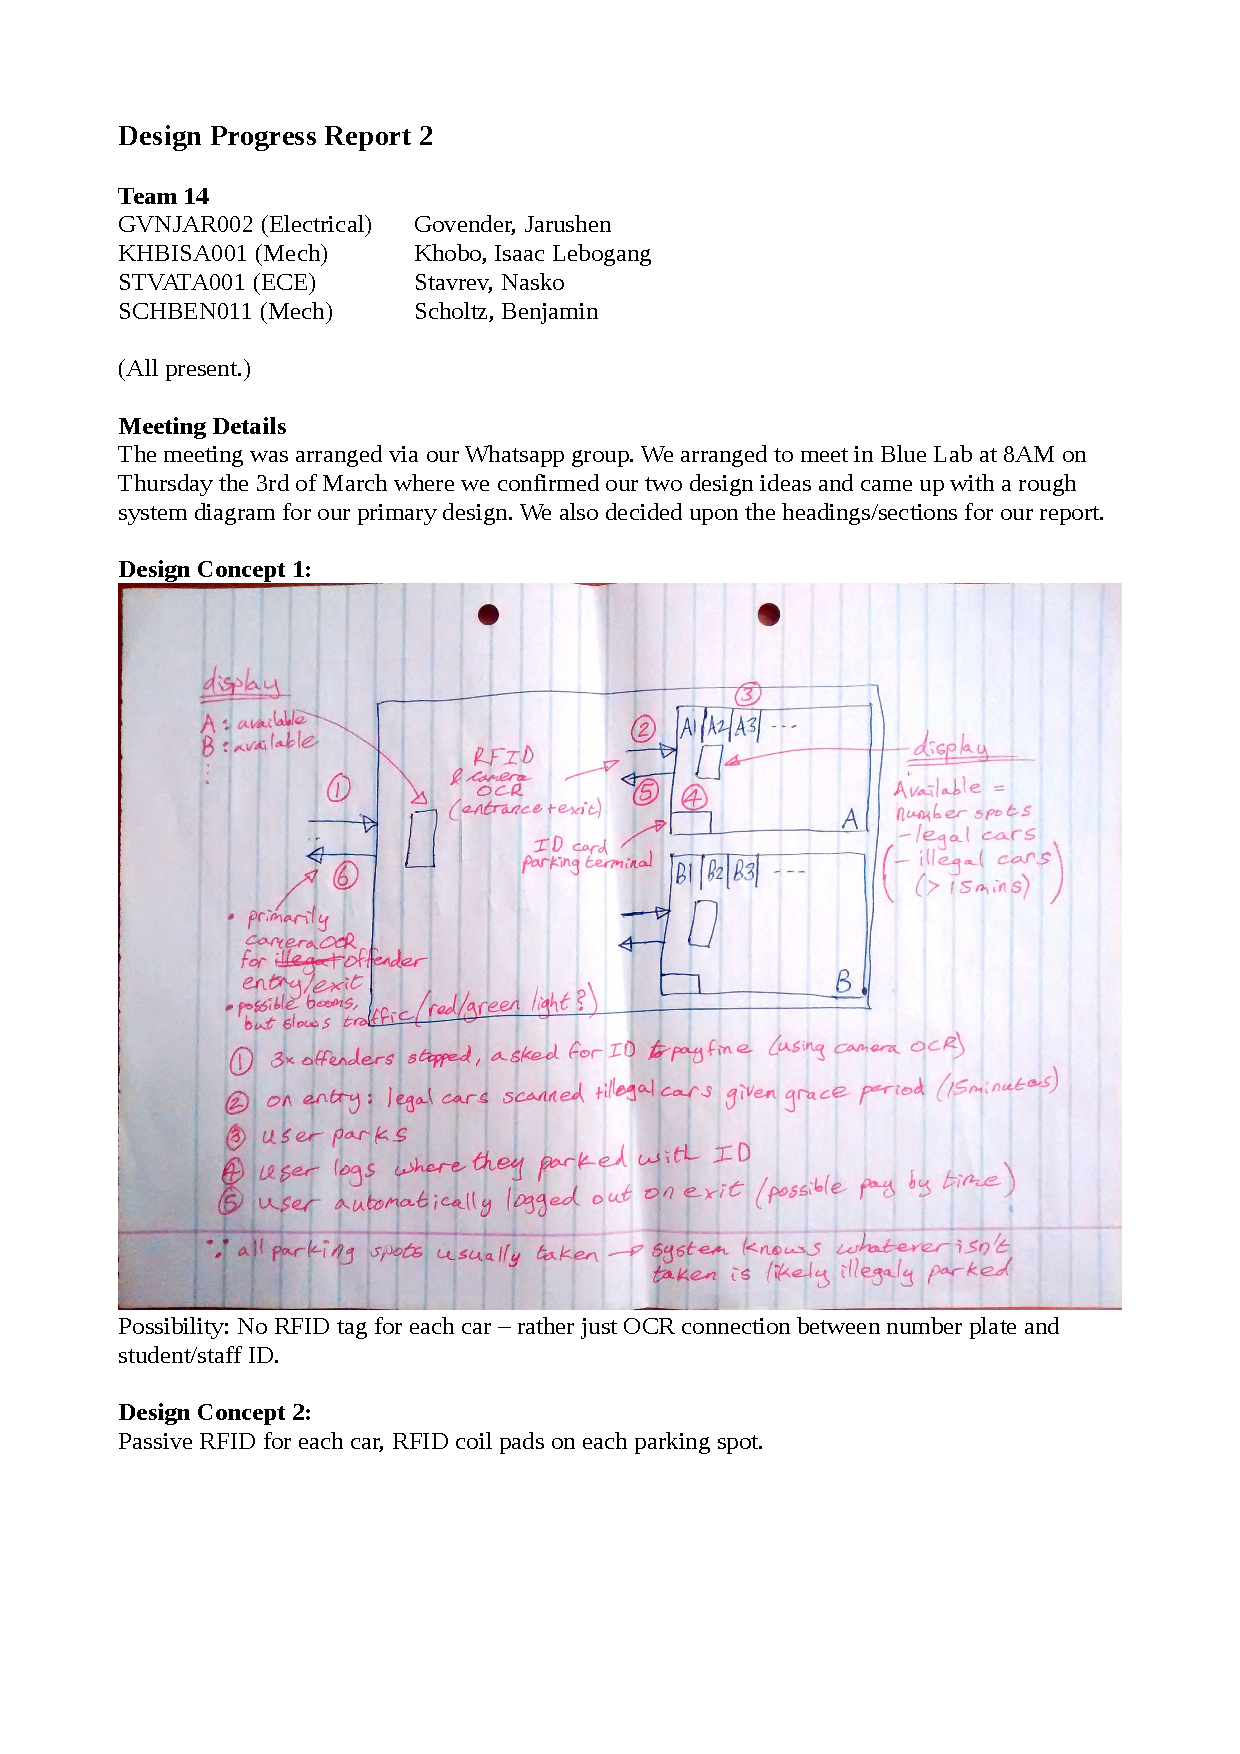
\includepdf[pages=-]{meeting/report2-ben.pdf}

\newpage
\vspace*{\fill}
\begin{center}
\subsection*{Progress Report 3}
\end{center}
\vspace*{\fill}
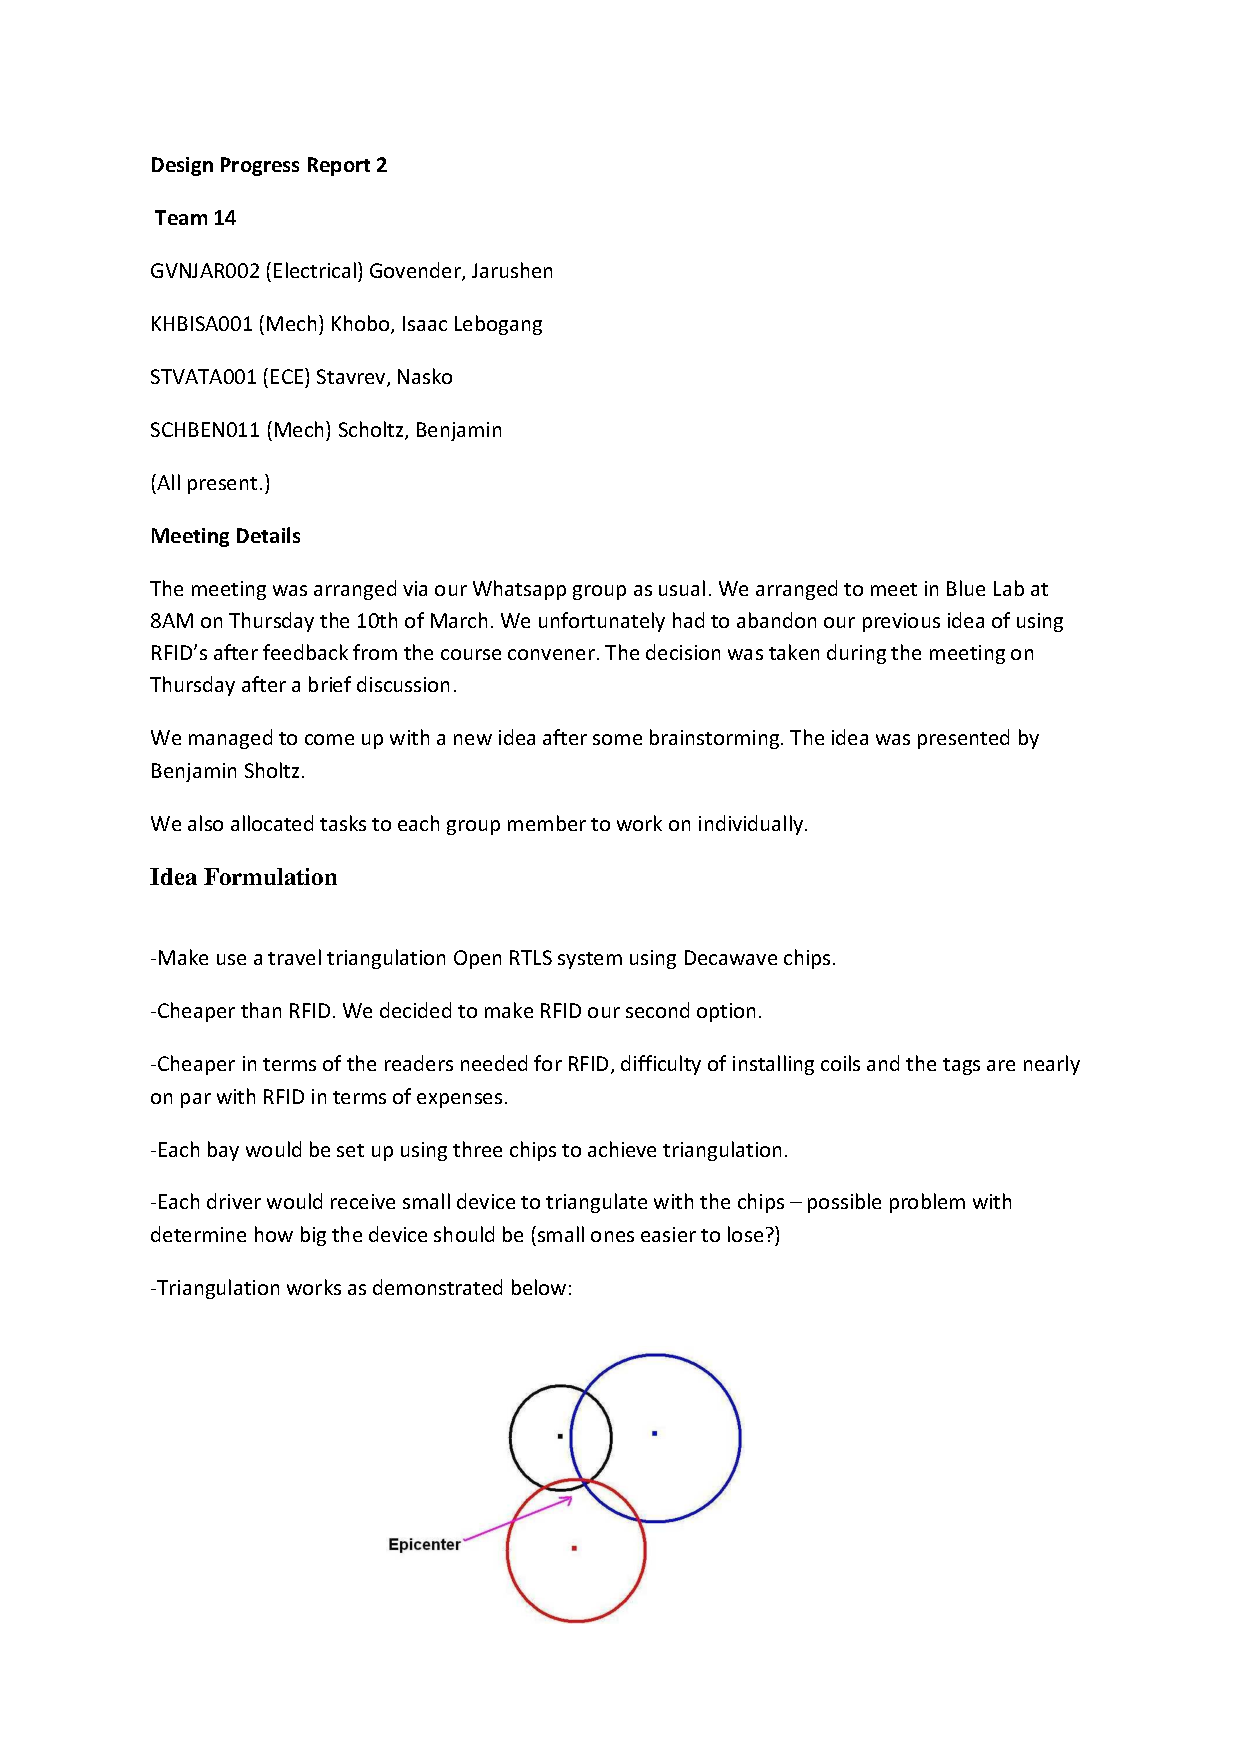
\includepdf[pages=-]{meeting/report3-jarushen.pdf}

\newpage
\vspace*{\fill}
\begin{center}
\subsection*{Progress Report 4}
\end{center}
\vspace*{\fill}
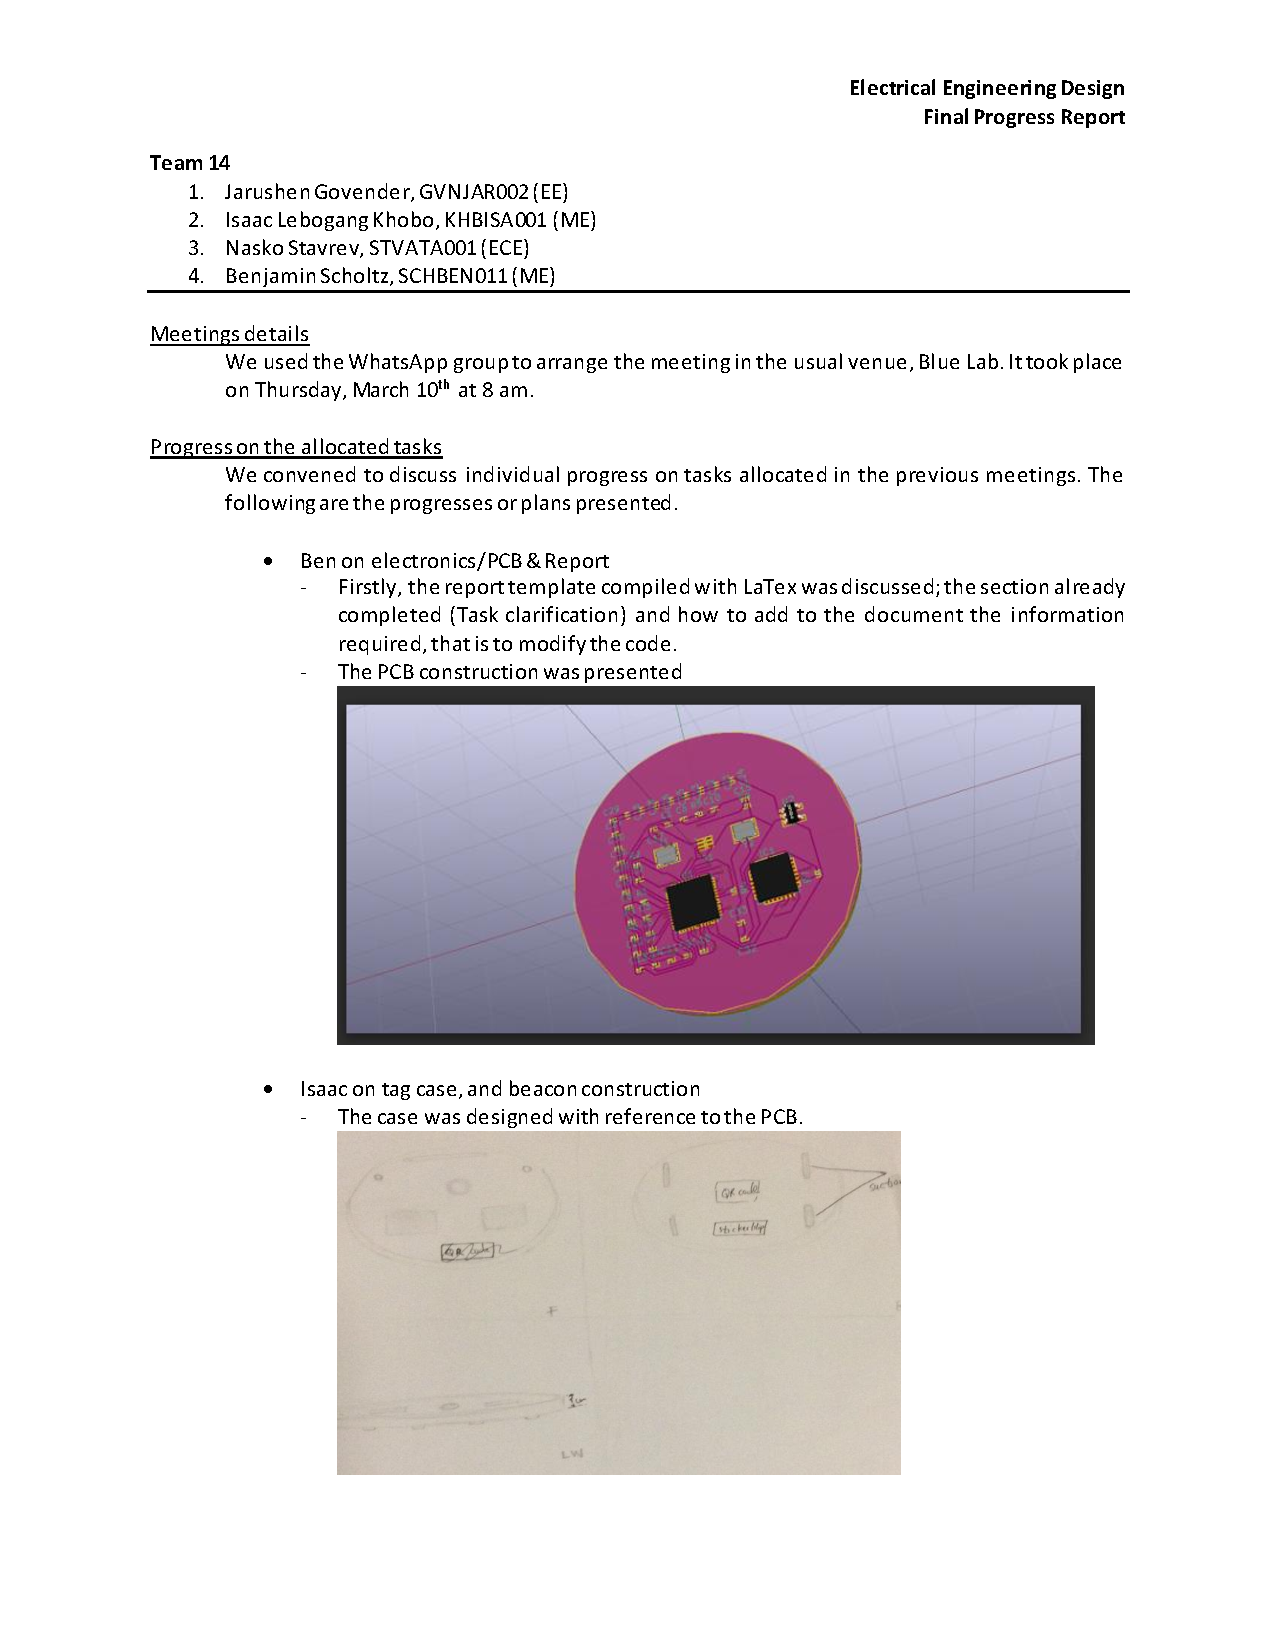
\includepdf[pages=-]{meeting/report4-isaac.pdf}

\newpage
\vspace*{\fill}
\begin{center}
\subsection*{Appendix C: Tag Bill of Materials and Unit Cost}
\end{center}
\vspace*{\fill}
\addcontentsline{toc}{section}{Appendix C: Tag Bill of Materials and Unit Cost}

\begin{landscape}
\begin{table}[]
\centering
\tiny
\caption{Tag Bill of Materials and Unit Cost Analysis}
\label{bom}
\begin{tabular}{llllllll}
\textbf{Ref}   & \textbf{Type} & \textbf{Value}             & \textbf{Footprint}              & \textbf{Part No. (Mouser default)}   & \textbf{Cost (US\$)} & \textbf{Outlay} & \textbf{Cost Outlay} \\
C4             & Capacitor     & 0.1uF                      & Capacitors\_SMD:C\_0201         & 81-GRM033R60J104KE19                 & 0.005                & 15000           & 75                   \\
C6             & Capacitor     & 0.1uF                      & Capacitors\_SMD:C\_0201         & 81-GRM033R60J104KE19                 & 0.005                & 15000           & 75                   \\
R2             & Resistor      & 100K                       & Resistors\_SMD:R\_0201          & 660-RK73H1HTTC1003F                  & 0.01                 & 15000           & 150                  \\
C31            & Capacitor     & 0.1uF                      & Capacitors\_SMD:C\_0201         & 81-GRM033R60J104KE19                 & 0.005                & 15000           & 75                   \\
C30            & Capacitor     & 4.7uF                      & Capacitors\_SMD:C\_0201         & 963-JMK063BJ474KP-F                  & 0.041                & 15000           & 615                  \\
C29            & Capacitor     & 0.1uF                      & Capacitors\_SMD:C\_0201         & 81-GRM033R60J104KE19                 & 0.005                & 15000           & 75                   \\
C28            & Capacitor     & 0.1uF                      & Capacitors\_SMD:C\_0201         & 81-GRM033R60J104KE19                 & 0.005                & 15000           & 75                   \\
C27            & Capacitor     & 0.1uF                      & Capacitors\_SMD:C\_0201         & 81-GRM033R60J104KE19                 & 0.005                & 15000           & 75                   \\
C26            & Capacitor     & 0.1uF                      & Capacitors\_SMD:C\_0201         & 81-GRM033R60J104KE19                 & 0.005                & 15000           & 75                   \\
C25            & Capacitor     & 1000pF                     & Capacitors\_SMD:C\_0201         & 81-GRM033R71E102KA1D                 & 0.004                & 15000           & 60                   \\
C24            & Capacitor     & 330pF                      & Capacitors\_SMD:C\_0201         & 81-GRM033R71E331KA1D                 & 0.004                & 15000           & 60                   \\
C23            & Capacitor     & 10pF                       & Capacitors\_SMD:C\_0201         & 81-GRM0335C1E100JA1D                 & 0.003                & 15000           & 45                   \\
C22            & Capacitor     & 0.1uF                      & Capacitors\_SMD:C\_0201         & 81-GRM033R60J104KE19                 & 0.005                & 15000           & 75                   \\
C21            & Capacitor     & 330pF                      & Capacitors\_SMD:C\_0201         & 81-GRM033R71E331KA1D                 & 0.004                & 15000           & 60                   \\
C20            & Capacitor     & 10pF                       & Capacitors\_SMD:C\_0201         & 81-GRM0335C1E100JA1D                 & 0.003                & 15000           & 45                   \\
C19            & Capacitor     & 0.1uF                      & Capacitors\_SMD:C\_0201         & 81-GRM033R60J104KE19                 & 0.005                & 15000           & 75                   \\
C18            & Capacitor     & 47uF                       & Capacitors\_SMD:C\_0201         & 581-TPSC476K016R0350                 & 0.206                & 15000           & 3090                 \\
C15            & Capacitor     & 0.1uF                      & Capacitors\_SMD:C\_0201         & 81-GRM033R60J104KE19                 & 0.005                & 15000           & 75                   \\
C17            & Capacitor     & 0.1uF                      & Capacitors\_SMD:C\_0201         & 81-GRM033R60J104KE19                 & 0.005                & 15000           & 75                   \\
C16            & Capacitor     & 0.1uF                      & Capacitors\_SMD:C\_0201         & 81-GRM033R60J104KE19                 & 0.005                & 15000           & 75                   \\
T1             & Transformer   & TRANSFO4                   & footprints:HHM1595A1            & 810-HHM1595A1                        & 0.362                & 15000           & 5430                 \\
C14            & Capacitor     & 0.1uF                      & Capacitors\_SMD:C\_0201         & 81-GRM033R60J104KE19                 & 0.005                & 15000           & 75                   \\
R6             & Resistor      & 270                        & Resistors\_SMD:R\_0201          & 667-ERJ-1GNF2700C                    & 0.005                & 15000           & 75                   \\
C12            & Capacitor     & 820pF                      & Capacitors\_SMD:C\_0201         & 81-GRM033R71E821KA1D                 & 0.004                & 15000           & 60                   \\
C13            & Capacitor     & 18pF                       & Capacitors\_SMD:C\_0201         & 581-02013A180GAT2A                   & 0.099                & 15000           & 1485                 \\
C11            & Capacitor     & 0.1uF                      & Capacitors\_SMD:C\_0201         & 81-GRM033R60J104KE19                 & 0.005                & 15000           & 75                   \\
C9             & Capacitor     & 1.2pF                      & Capacitors\_SMD:C\_0201         & 810-C0603C0G1E1R2BTQ                 & 0.02                 & 15000           & 300                  \\
R3             & Resistor      & 16k                        & Resistors\_SMD:R\_0201          & 667-ERJ-1GEJ163C                     & 0.004                & 15000           & 60                   \\
C8             & Capacitor     & 27pF                       & Capacitors\_SMD:C\_0201         & 81-GRM0335C1E270JA1D                 & 0.004                & 15000           & 60                   \\
C7             & Capacitor     & 0.1uF                      & Capacitors\_SMD:C\_0201         & 81-GRM033R60J104KE19                 & 0.005                & 15000           & 75                   \\
R1             & Resistor      & 11k 1\%                    & Resistors\_SMD:R\_0201          & 71-CRCW020111K0FKED                  & 0.026                & 15000           & 390                  \\
C5             & Capacitor     & 0.1uF                      & Capacitors\_SMD:C\_0201         & 81-GRM033R60J104KE19                 & 0.005                & 15000           & 75                   \\
C3             & Capacitor     & 0.1uF                      & Capacitors\_SMD:C\_0201         & 81-GRM033R60J104KE19                 & 0.005                & 15000           & 75                   \\
R4             & Resistor      & 10k                        & Resistors\_SMD:R\_0201          & 603-RC0201FR-0710KL                  & 0.004                & 15000           & 60                   \\
R5             & Resistor      & 10k                        & Resistors\_SMD:R\_0201          & 603-RC0201FR-0710KL                  & 0.004                & 15000           & 60                   \\
C2             & Capacitor     & 10pF                       & Capacitors\_SMD:C\_0201         & 81-GRM0335C1E100JA1D                 & 0.003                & 15000           & 45                   \\
C1             & Capacitor     & 10pF                       & Capacitors\_SMD:C\_0201         & 81-GRM0335C1E100JA1D                 & 0.003                & 15000           & 45                   \\
Y1             & Crystal       & 38.4MHz                    & Crystals:FA238-TSX3225          & ABM10-165-38.400MHz-T3               & 0.667                & 15000           & 10005                \\
C10            & Capacitor     & 0.1uF                      & Capacitors\_SMD:C\_0201         & 81-GRM033R60J104KE19                 & 0.005                & 15000           & 75                   \\
U1             & Transciever   & DW1000                     & Housings\_DFN\_QFN:QFN-48       & 1479-1001-2-ND                       & 8.8726               & 15000           & 133089               \\
U2             & DC-DC         & TPS62203DBV                & SMD:SOT-23-5                    & 595-TPS62203DBVR                     & 0.542                & 15000           & 8130                 \\
U3             & DC-DC         & TPS62203DBV                & SMD:SOT-23-5                    & 595-TPS62203DBVR                     & 0.542                & 15000           & 8130                 \\
C34            & Capacitor     & 4.7uF                      & Capacitors\_SMD:C\_0201         & 963-JMK063BJ474KP-F                  & 0.041                & 15000           & 615                  \\
L1             & Inductor      & 10uH                       & Inductors:Inductor\_1212        & 81-LQH3NPN100MM0L                    & 0.132                & 15000           & 1980                 \\
C35            & Capacitor     & 10uF                       & Capacitors\_SMD:C\_0201         & 80-T491C106K016                      & 0.102                & 15000           & 1530                 \\
P1             & Connector     & CONN\_01X02                & Connectors\_Molex               & See note.                            & 0.5                  & 15000           & 7500                 \\
P2             & Antenna       & Antenna                    & PCB Chip Antenna                & 963-AH086M555003-T                   & 0.803                & 15000           & 12045                \\
IC1            & Micro.        & ATMEGA328P-MM              & DFN\_QFN:QFN-28                 & 556-ATMEGA328P-MMH                   & 1.89                 & 15000           & 28350                \\
R7             & Resistor      & 10k                        & Resistors\_SMD:R\_0201          & 603-RC0201FR-0710KL                  & 0.004                & 15000           & 60                   \\
Y2             & Crystal       & 16MHz                      & Crystals:crystal\_FA238-TSX3225 & 732-TX325-16F09Z-AC3                 & 0.278                & 15000           & 4170                 \\
C32            & Capacitor     & 22pF                       & Capacitors\_SMD:C\_0201         & 810-C0603C0G1H220J                   & 0.004                & 15000           & 60                   \\
C33            & Capacitor     & 22pF                       & Capacitors\_SMD:C\_0201         & 810-C0603C0G1H220J                   & 0.004                & 15000           & 60                   \\
               &               &                            &                                 & \textbf{Total Capital Outlay (ZAR):} &                      &                 & \textbf{3558254.88}  \\
               &               &                            &                                 & \textbf{Unit Cost (ZAR):}            &                      &                 & \textbf{237.216992}  \\
               &               &                            &                                 &                                      &                      &                 &                      \\
\textbf{Notes} &               &                            &                                 &                                      &                      &                 &                      \\
P1             & Connector     & Part No.: Diff. Footprint. &                                 &                                      &                      &                 &                      \\
C35            & Capacitor     & Footprint: 2412            &                                 &                                      &                      &                 &                      \\
U1             & Transciever   & Supplier: Digikey          &                                 &                                      &                      &                 &                     
\end{tabular}
\end{table}
\end{landscape}

\end{document}

%----------------------------------------------------------------------------


